\index{Kunzmann, Ute}

\paragraph{Research Team}
Ute Kunzmann (Professor), David Richter (Doctoral Fellow).

 The concept of emotional competence has received widespread attention in several psychological disciplines and various definitions have recently been suggested, differing in terms of content and breadth. Ute Kunzmann and her collaborators have considered emotional competence as a multidimensional concept that covers several distinct facets, including the capacity to spontaneously react to emotion-arousing events with the appropriate emotion, the ability to voluntarily regulate one's own emotions, and the ability to accurately detect other's emotions.
 
 Keeping in mind that people's subjective evaluations of what they can do are sometimes not accurate reflections of their ``objective'' competencies, Ute Kunzmann has begun to design and conduct well-controlled experimental studies in which emotions and emotional abilities can be observed in vivo. In these studies, adults of different ages are exposed to the same emotionally challenging tasks and their subsequent cognitive and emotional reactions are observed objectively. Evidence from this research is meant to supplement the findings from studies employing self-report questionnaires and performance-based tests of emotional competence. 

Findings from the Kunzmann's and her collaborators' laboratories strongly support the general propositions of life-span developmental psychology described above. For example, there is robust evidence for multidirectionality in the realm of emotional reactivity. Whereas autonomic reactions seem to decline with age, subjective reactions remain stable. Furthermore, this pattern of age differences is not fixed but at least partly determined by contextual factors such as the age-relevance of the emotion-arousing event. When being exposed to emotion-evoking themes that are particularly salient in old age, older adult's reactions are greater or just as large than those of young adults - even on the level of autonomic activity.  

Ute Kunzmann and her collaborators at the University of California, Berkeley also provided first performance-based evidence that the ability to regulate one's own emotional reactions on command remains unchanged over adulthood and old age. This evidence refers to one particular form of emotion regulation, that is, the ability to voluntarily up- and down regulate one's facial expressions. Given that emotion regulation comprises multiple forms, the question arises of whether the current evidence can be generalized to other forms of emotion regulation (e.g., the ability to re-evaluate negative experiences so that they become less threatening to the self). An experimental study that Ute Kunzmann designed together with Prof. Fredda Blanchard Fields at the Georgia Institute of Technology, Atlanta will begin to address this question in the near future.

\null
\textbf{Research Highlights 2006}

\textit{Study on Empathic Accuracy: First Results}

 Our research activities during the last months have focused on yet another emotional ability, namely, the \textit{ability to accurately perceive other people's emotions} (i.e., empathic accuracy). As is true for so many resource-demanding and effortful functions, the empirical evidence generally suggests that young adults outperform older adults in tasks assessing this ability. However, a serious limitation of the typical paradigm used to study age differences in empathic accuracy is its lack of ecological validity. Participants are typically asked to recognize emotions from still photographs of faces, which provide very little information about the evaluated persons. Moreover, emotions are typically posed rather than truly experienced. Studying emotion recognition via tasks that are less stripped down in terms of familiarity and meaningfulness might yield a very different picture about age differences in this ability.  

 To test this proposal, Ute Kunzmann and David Richter conducted a study with more contextualized empathic accuracy tasks in our lab. Instead of presenting to young and old adults photographs of people posing prototypical emotions, they presented eight short film clips each dealing with a person as he or she was talking about an emotionally engaging issue. The to be evaluated people experienced real and authentic emotions while talking. To study the role of motivational factors, the age relevance of the topics the videotaped people were talking about was manipulated. One topic was of particular relevance to older people and dealt with age-related losses. A second topic was of particular relevance to young people and dealt with an adventurous and risky life transition. 

 As can be seen in Figure \ref{fig1:profUteKunzmann}, the age-related decline in emotion recognition found in earlier studies was only evident in situations that were of minor relevance to older people. In contrast, there was no age difference in performance level when the task was to accurately evaluate the emotions of a person who talked about a topic that was particularly relevant in old age. Two conclusions from this work are that age-related decline in resource-demanding processes may be limited to tasks and contexts that are of little relevance to older people and that motivational factors can offset age-related deficits. Ute Kunzmann and David Richter organized a symposium with the title ``lifespan development of emotions and emotional competencies'' at the 45th Congress of the German Society for Psychology in September 2006 in the context of which they presented their latest findings. In addition, they are about to submit a grant proposal to the German Research Foundation that will allow them to test additional moderators of the relationship between age and empathic accuracy.

\begin{figure}[htb]
  \begin{center}
    \resizebox{0.5\textwidth}{!}{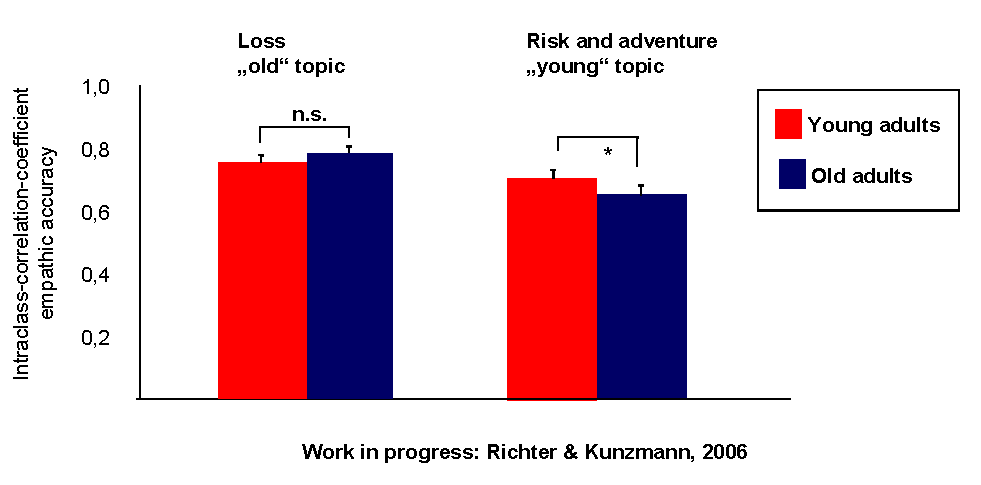
\includegraphics{profUteKunzmann-fig1}}
    \caption{Age differences in empathic accuracy: Age relevance matters.}
    \label{fig1:profUteKunzmann}
  \end{center}
\end{figure}



\textit{Research Network from the German Research Foundation}

 Another research highlight of the last year was a first meeting of a research network funded by the German Research Foundation (faculty member: Ute Kunzmann; student member: David Richter). The network consists of German researchers who study the differential and general development of emotions and emotional competencies. The network members (1/3 faculty and 2/3 graduate students) will hold two meetings per year for a period of three years. The meetings will be designed (a) to facilitate exchange of ideas and expertise, (b) to discuss research with invited internationally distinguished emotion researchers (two guests per meeting), and (c) to develop plans for future collaborative research projects.

\paragraph{Collaborations}
\begin{itemize}
\item Georgia Institute of Technology, Atlanta, USA \\ Prof. Fredda H. Blanchard-Fields, PhD
\item University of California, Berkeley, USA \\ Prof. Robert W. Levenson, PhD
\item University of Geneva, Geneva, CH \\ Prof. Gisela Labouvie-Vief, PhD
\end{itemize}

\begin{bibunit}[apalike]
\nocite{*}
\putbib[profUteKuzmann1]
\end{bibunit}



\paragraph{Grants}

\begin{itemize}
	\item BMBF (PI: JCLL). U. Kunzmann, U.M. Staudinger: subproject ``Images of Aging'' within the joint research project ``Effects of Matches/Mismatches between Aspects of Human and Social Capital, Corporate Strategy and Work Organization on the Physical and Mental Well-Being of Employees''. 
\end{itemize}

